\documentclass{ximera}  


%\usepackage{todonotes}
%\usepackage{mathtools} %% Required for wide table Curl and Greens
%\usepackage{cuted} %% Required for wide table Curl and Greens
\newcommand{\todo}{}

\usepackage{esint} % for \oiint
\ifxake%%https://math.meta.stackexchange.com/questions/9973/how-do-you-render-a-closed-surface-double-integral
\renewcommand{\oiint}{{\large\bigcirc}\kern-1.56em\iint}
\fi


\graphicspath{
  {./}
  {jpg}
  {ximeraTutorial/}
  {basicPhilosophy/}
  {functionsOfSeveralVariables/}
  {normalVectors/}
  {lagrangeMultipliers/}
  {vectorFields/}
  {greensTheorem/}
  {shapeOfThingsToCome/}
  {dotProducts/}
  {partialDerivativesAndTheGradientVector/}
  {../productAndQuotientRules/exercises/}
  {../motionAndPathsInSpace/exercises/}
  {../normalVectors/exercisesParametricPlots/}
  {../continuityOfFunctionsOfSeveralVariables/exercises/}
  {../partialDerivativesAndTheGradientVector/exercises/}
  {../directionalDerivativeAndChainRule/exercises/}
  {../commonCoordinates/exercisesCylindricalCoordinates/}
  {../commonCoordinates/exercisesSphericalCoordinates/}
  {../greensTheorem/exercisesCurlAndLineIntegrals/}
  {../greensTheorem/exercisesDivergenceAndLineIntegrals/}
  {../shapeOfThingsToCome/exercisesDivergenceTheorem/}
  {../greensTheorem/}
  {../shapeOfThingsToCome/}
  {../separableDifferentialEquations/exercises/}
  {vectorFields/}
}

\newcommand{\mooculus}{\textsf{\textbf{MOOC}\textnormal{\textsf{ULUS}}}}

\usepackage{tkz-euclide}\usepackage{tikz}
\usepackage{tikz-cd}
\usetikzlibrary{arrows}
\tikzset{>=stealth,commutative diagrams/.cd,
  arrow style=tikz,diagrams={>=stealth}} %% cool arrow head
\tikzset{shorten <>/.style={ shorten >=#1, shorten <=#1 } } %% allows shorter vectors

\usetikzlibrary{backgrounds} %% for boxes around graphs
\usetikzlibrary{shapes,positioning}  %% Clouds and stars
\usetikzlibrary{matrix} %% for matrix
\usepgfplotslibrary{polar} %% for polar plots
\usepgfplotslibrary{fillbetween} %% to shade area between curves in TikZ
\usetkzobj{all}
\usepackage[makeroom]{cancel} %% for strike outs
%\usepackage{mathtools} %% for pretty underbrace % Breaks Ximera
%\usepackage{multicol}
\usepackage{pgffor} %% required for integral for loops



%% http://tex.stackexchange.com/questions/66490/drawing-a-tikz-arc-specifying-the-center
%% Draws beach ball
\tikzset{pics/carc/.style args={#1:#2:#3}{code={\draw[pic actions] (#1:#3) arc(#1:#2:#3);}}}



\usepackage{array}
\setlength{\extrarowheight}{+.1cm}
\newdimen\digitwidth
\settowidth\digitwidth{9}
\def\divrule#1#2{
\noalign{\moveright#1\digitwidth
\vbox{\hrule width#2\digitwidth}}}





\newcommand{\RR}{\mathbb R}
\newcommand{\R}{\mathbb R}
\newcommand{\N}{\mathbb N}
\newcommand{\Z}{\mathbb Z}

\newcommand{\sagemath}{\textsf{SageMath}}


%\renewcommand{\d}{\,d\!}
\renewcommand{\d}{\mathop{}\!d}
\newcommand{\dd}[2][]{\frac{\d #1}{\d #2}}
\newcommand{\pp}[2][]{\frac{\partial #1}{\partial #2}}
\renewcommand{\l}{\ell}
\newcommand{\ddx}{\frac{d}{\d x}}

\newcommand{\zeroOverZero}{\ensuremath{\boldsymbol{\tfrac{0}{0}}}}
\newcommand{\inftyOverInfty}{\ensuremath{\boldsymbol{\tfrac{\infty}{\infty}}}}
\newcommand{\zeroOverInfty}{\ensuremath{\boldsymbol{\tfrac{0}{\infty}}}}
\newcommand{\zeroTimesInfty}{\ensuremath{\small\boldsymbol{0\cdot \infty}}}
\newcommand{\inftyMinusInfty}{\ensuremath{\small\boldsymbol{\infty - \infty}}}
\newcommand{\oneToInfty}{\ensuremath{\boldsymbol{1^\infty}}}
\newcommand{\zeroToZero}{\ensuremath{\boldsymbol{0^0}}}
\newcommand{\inftyToZero}{\ensuremath{\boldsymbol{\infty^0}}}



\newcommand{\numOverZero}{\ensuremath{\boldsymbol{\tfrac{\#}{0}}}}
\newcommand{\dfn}{\textbf}
%\newcommand{\unit}{\,\mathrm}
\newcommand{\unit}{\mathop{}\!\mathrm}
\newcommand{\eval}[1]{\bigg[ #1 \bigg]}
\newcommand{\seq}[1]{\left( #1 \right)}
\renewcommand{\epsilon}{\varepsilon}
\renewcommand{\phi}{\varphi}


\renewcommand{\iff}{\Leftrightarrow}

\DeclareMathOperator{\arccot}{arccot}
\DeclareMathOperator{\arcsec}{arcsec}
\DeclareMathOperator{\arccsc}{arccsc}
\DeclareMathOperator{\si}{Si}
\DeclareMathOperator{\scal}{scal}
\DeclareMathOperator{\sign}{sign}


%% \newcommand{\tightoverset}[2]{% for arrow vec
%%   \mathop{#2}\limits^{\vbox to -.5ex{\kern-0.75ex\hbox{$#1$}\vss}}}
\newcommand{\arrowvec}[1]{{\overset{\rightharpoonup}{#1}}}
%\renewcommand{\vec}[1]{\arrowvec{\mathbf{#1}}}
\renewcommand{\vec}[1]{{\overset{\boldsymbol{\rightharpoonup}}{\mathbf{#1}}}\hspace{0in}}

\newcommand{\point}[1]{\left(#1\right)} %this allows \vector{ to be changed to \vector{ with a quick find and replace
\newcommand{\pt}[1]{\mathbf{#1}} %this allows \vec{ to be changed to \vec{ with a quick find and replace
\newcommand{\Lim}[2]{\lim_{\point{#1} \to \point{#2}}} %Bart, I changed this to point since I want to use it.  It runs through both of the exercise and exerciseE files in limits section, which is why it was in each document to start with.

\DeclareMathOperator{\proj}{\mathbf{proj}}
\newcommand{\veci}{{\boldsymbol{\hat{\imath}}}}
\newcommand{\vecj}{{\boldsymbol{\hat{\jmath}}}}
\newcommand{\veck}{{\boldsymbol{\hat{k}}}}
\newcommand{\vecl}{\vec{\boldsymbol{\l}}}
\newcommand{\uvec}[1]{\mathbf{\hat{#1}}}
\newcommand{\utan}{\mathbf{\hat{t}}}
\newcommand{\unormal}{\mathbf{\hat{n}}}
\newcommand{\ubinormal}{\mathbf{\hat{b}}}

\newcommand{\dotp}{\bullet}
\newcommand{\cross}{\boldsymbol\times}
\newcommand{\grad}{\boldsymbol\nabla}
\newcommand{\divergence}{\grad\dotp}
\newcommand{\curl}{\grad\cross}
%\DeclareMathOperator{\divergence}{divergence}
%\DeclareMathOperator{\curl}[1]{\grad\cross #1}
\newcommand{\lto}{\mathop{\longrightarrow\,}\limits}

\renewcommand{\bar}{\overline}

\colorlet{textColor}{black}
\colorlet{background}{white}
\colorlet{penColor}{blue!50!black} % Color of a curve in a plot
\colorlet{penColor2}{red!50!black}% Color of a curve in a plot
\colorlet{penColor3}{red!50!blue} % Color of a curve in a plot
\colorlet{penColor4}{green!50!black} % Color of a curve in a plot
\colorlet{penColor5}{orange!80!black} % Color of a curve in a plot
\colorlet{penColor6}{yellow!70!black} % Color of a curve in a plot
\colorlet{fill1}{penColor!20} % Color of fill in a plot
\colorlet{fill2}{penColor2!20} % Color of fill in a plot
\colorlet{fillp}{fill1} % Color of positive area
\colorlet{filln}{penColor2!20} % Color of negative area
\colorlet{fill3}{penColor3!20} % Fill
\colorlet{fill4}{penColor4!20} % Fill
\colorlet{fill5}{penColor5!20} % Fill
\colorlet{gridColor}{gray!50} % Color of grid in a plot

\newcommand{\surfaceColor}{violet}
\newcommand{\surfaceColorTwo}{redyellow}
\newcommand{\sliceColor}{greenyellow}




\pgfmathdeclarefunction{gauss}{2}{% gives gaussian
  \pgfmathparse{1/(#2*sqrt(2*pi))*exp(-((x-#1)^2)/(2*#2^2))}%
}


%%%%%%%%%%%%%
%% Vectors
%%%%%%%%%%%%%

%% Simple horiz vectors
\renewcommand{\vector}[1]{\left\langle #1\right\rangle}


%% %% Complex Horiz Vectors with angle brackets
%% \makeatletter
%% \renewcommand{\vector}[2][ , ]{\left\langle%
%%   \def\nextitem{\def\nextitem{#1}}%
%%   \@for \el:=#2\do{\nextitem\el}\right\rangle%
%% }
%% \makeatother

%% %% Vertical Vectors
%% \def\vector#1{\begin{bmatrix}\vecListA#1,,\end{bmatrix}}
%% \def\vecListA#1,{\if,#1,\else #1\cr \expandafter \vecListA \fi}

%%%%%%%%%%%%%
%% End of vectors
%%%%%%%%%%%%%

%\newcommand{\fullwidth}{}
%\newcommand{\normalwidth}{}



%% makes a snazzy t-chart for evaluating functions
%\newenvironment{tchart}{\rowcolors{2}{}{background!90!textColor}\array}{\endarray}

%%This is to help with formatting on future title pages.
\newenvironment{sectionOutcomes}{}{}



%% Flowchart stuff
%\tikzstyle{startstop} = [rectangle, rounded corners, minimum width=3cm, minimum height=1cm,text centered, draw=black]
%\tikzstyle{question} = [rectangle, minimum width=3cm, minimum height=1cm, text centered, draw=black]
%\tikzstyle{decision} = [trapezium, trapezium left angle=70, trapezium right angle=110, minimum width=3cm, minimum height=1cm, text centered, draw=black]
%\tikzstyle{question} = [rectangle, rounded corners, minimum width=3cm, minimum height=1cm,text centered, draw=black]
%\tikzstyle{process} = [rectangle, minimum width=3cm, minimum height=1cm, text centered, draw=black]
%\tikzstyle{decision} = [trapezium, trapezium left angle=70, trapezium right angle=110, minimum width=3cm, minimum height=1cm, text centered, draw=black]




 
\title{Power Transfer on a transmission line} 
\author{Milica Markovic} 
\outcome{Explain why is the impedance matching needed
 How real power changes from the input to the output of a lossless transmission line. Explain how maximum available power from the generator affects power on the transmission line. Explain how minimum reflection from the generator affects power on a transmission line. Explain how minimum reflection from the load affects power on a transmission line.}
\begin{document}  
\begin{abstract}  

\end{abstract}  
\maketitle    

\subsection*{Power Transfer on a Transmission Line}

Power on a transmission line can be found similarly to the derivation in the previous section. It is just that now, the total voltage is the sum of the forward-going and reflected voltage, and the total current is the sum of the forward and reflected current. 


\begin{eqnarray}
\tilde{V}(z)=\tilde{V}_0^+ e^{-\gamma z} + \tilde{V}_0^- e^{\gamma z}\label{eq4a} \\
I(z)=\tilde{I}_0^+ e^{-\gamma z} + \tilde{I}_0^- e^{\gamma z}\label{eq5a}
\end{eqnarray}

Where $\tilde{V}^+(z)=\tilde{V}_0^+ e^{-\gamma z} $ is the phasor of forward voltage anywhere on the line, and $\tilde{V}^-(z)=\tilde{V}_0^- e^{\gamma z}$ is the phasor of reflected voltage anywhere on the line. $\tilde{V}_0^+$ is the phasor of forward voltage at the load, where z=0, and  $\tilde{V}_0^-$ is the phasor of reflected voltage at the load, where z=0.  The currents are similarly named. If the line is lossless, then the attenuation coefficient $\alpha=0$ and $\gamma= \alpha + j \beta = j \beta$, so the equations become



\begin{eqnarray}
\tilde{V}(z)=\tilde{V}_0^+ e^{-j\beta z} + \tilde{V}_0^- e^{j\beta z}\label{eq4} \\
I(z)=\tilde{I}_0^+ e^{-j\beta z} + \tilde{I}_0^- e^{j\beta z}\label{eq5}
\end{eqnarray}

If we define a phasor of reflection coefficient at the load as $\Gamma =\frac{\tilde{V}^-_0(z)}{\tilde{V}^+_0(z)}$, and define the transmission-line impedance as $Z_0=\frac{\tilde{V}_0^+}{\tilde{I}_0^+}=-\frac{\tilde{V}_0^-}{\tilde{I}_0^-}$ then the equations become

\begin{eqnarray}
\tilde{V}(z)=\tilde{V}_0^+ e^{-j\beta z} + \Gamma \tilde{V}_0^+ e^{j\beta z}\label{eq4b} \\
I(z)=\frac{\tilde{V}_0^+}{Z_0} e^{-j\beta z} - \Gamma \frac{\tilde{V}_0^+}{Z_0} e^{j\beta z}\label{eq5b}
\end{eqnarray}

By multiplying phasors above, we get the phasor of the average real incident (forward) $P_i$ and reflected power $P_r$ anywhere on the line.

\begin{eqnarray}
P_i=\frac{|\tilde{V}_0^+|^2}{2 Z_0} \\
P_r= |\Gamma|^2 \frac{|\tilde{V}_0^+|^2}{2 Z_0}
\end{eqnarray}

Total power delivered to the load is then  $P_L=P_i-P_r$

\begin{eqnarray}
P_L=\frac{|\tilde{V}_0^+|^2}{2 Z_0} - |\Gamma|^2 \frac{|\tilde{V}_0^+|^2}{2 Z_0} \\
P_L=\frac{|\tilde{V}_0^+|^2}{2 Z_0} (1-|\Gamma|^2 ) \label{eq:power}
\end{eqnarray}


\subsection{Maximizing power transfer on a transmission line}

Looking at Equation \ref{eq:power}, to maximize power delivered to the load $P_L$  , we have to maximize $|\tilde{V}_0^+|$, or minimize $Z_0$ and $|\Gamma|$. 


\begin{enumerate}
\item $Z_0$, the transmission-line impedance, is fixed if we are using a specific type of a coaxial cable as we have seen previously, typical impedances of coaxial cables are $50\Omega$, $75\Omega$, $300\Omega$. However, if we are using microstrip lines,  transmission line impedance can be part of the circuit design, and we can make $Z_0$ lower.
\item To minimize $|\Gamma|=\frac{\tilde{V}_0^-}{\tilde{V}_0^+} =\frac{Z_L-Z_0}{Z_L+Z_0}=0$ we have to make the reflected voltage (and power) zero by making the load impedance equal to the transmission line impedance $Z_L-Z_0=0$, or $Z_L=Z_0$. 
\item To maximize $|\tilde{V}_0^+|$, according to the maximum power transfer theorem, the input impedance to the transmission line has to be equal to the conjugate of the generator's impedance $Z_{in}=Z_{g}^*$. If the impedance of the generator is complex $Z_g=R_g+jX_g$, then the input impedance has to be $Z_{in}=R_g-jX_g$.
\end{enumerate}

There are two requirements, $Z_L=Z_0$ that minimizes reflected power,  and $Z_{in}=Z_g^*$ that maximizes forward power. The incident power on a  transmission line is given as

\begin{equation}
P_i=\frac{|\tilde{V}_0^+|^2}{2 Z_0}
\end{equation}


The forward going voltage on a transmission line depends on the input reflection coefficient, as shown in Equation \ref{eq:inputrefl}.

\begin{equation}
\tilde{V}_0^+=\frac{Z_0}{Z_0(1+\Gamma_{in})+Z_g(1-\Gamma_{in})}V_g e^{-j\beta l}\label{eq:inputrefl}
\end{equation}

$\Gamma_{in}=\frac{Zg-Z_0}{Zg+Z_0}$ is the reflection coefficient looking into the generator. It is interesting to see that when the generator impedance and transmission line impedance are the same (the reflection coefficient looking into the generator $\Gamma_{g}$ is zero), the forward-going voltage does not depend on the load impedance $Z_L$. Forward-going voltage is equal to $\tilde{V}_0^+=\frac{1}{2} V_g e^{j \beta z}$! 

When we turn on the generator, the generator sees a voltage divider: the generator's impedance $Z_g$ and only the transmission-line impedance $Z_0$ at the input of the line, not $Z_{in}$, because in the transient, the reflected voltage is not there to make the total impedance $Z_{in}$. The signal initially starts traveling toward the load, reflects off the load, and the reflected part of the voltage travels back to the generator. When the reflected part of the voltage arrives at the generator if $\Gamma_{g}\neq 0$, then the voltage wave reflects again from the generator, and the forward going voltage $\tilde{V}_0^+$ will change for the amount of that new reflection. However, if $\Gamma_{g}= 0$, the reflected wave will be absorbed by the generator, and no wave will be reflected. When input reflection coefficient is zero, $\Gamma_{g}=\frac{Zg-Z_0}{Zg+Z_0} = 0$. The generator impedance and the transmission-line impedance are the same.

Suppose we also select the reflected power to be zero by setting the load impedance to the transmission line impedance $Z_L=Z_0$. In that case, we have the best of both worlds, maximum power transfer and minimum reflection!


\section{Why we do impedance matching?}



We perform impedance matching to remove the reflected wave on the transmission line and maximize the power available from the generator.

Impedance matching is a technique that 
\begin{enumerate}
\item ensures maximum power transfer between the generator $V_g$ and the load $Z_L$, and 
\item minimizes the reflected power from the load. 
\end{enumerate}

To ensure that the voltage does not reflect from the generator, the generator's impedance should be the same as the transmission-line impedance. 


  When we insert the impedance matching circuit between the load $Z_L$ and the transmission line $Z_\circ$, as shown in Figure  \ref{eq:impmatchgen1} the input impedance presented to the generator and the transmission line from the impedance matching circuit is $Z_\circ$, and the impedance presented to the load impedance $Z_L$ will be $Z_L^*$. Our task is to add capacitors and inductors to the load $Z_L$ to make the input impedance equal to $Z_\circ$. We {\bf do not} want to use resistors in an impedance matching circuit because they will use some of the power that we need at $Z_L$.  

 

\begin{figure}[htbp]
\begin{center}
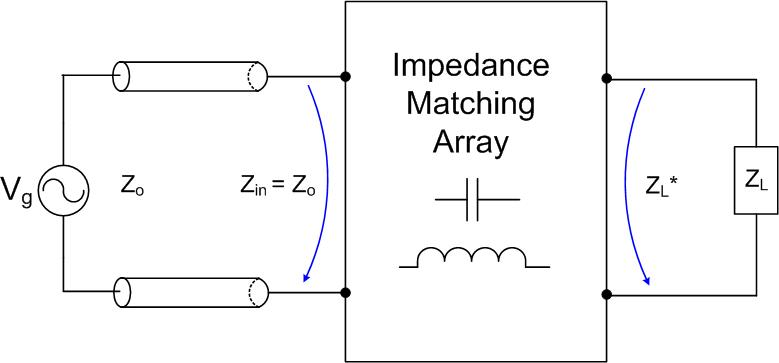
\includegraphics[scale=0.4]{../jpg/Impedancematching.jpg}
\end{center}
\caption{The result of impedance matching.}
\label{eq:impmatchgen1}
\end{figure}


\end{document} 

